\documentclass[a4paper,10pt]{article}
%\documentclass[a4paper,10pt]{scrartcl}

\usepackage{algorithm}
\usepackage{algorithmic}
\usepackage[utf8x]{inputenc}
\usepackage{verbatim}
\usepackage{amsmath}
\usepackage{bytefield}
\usepackage{graphicx}
\usepackage{morefloats}

\usepackage{anysize}
\marginsize{1in}{1in}{1in}{1in}

\title{Marvok-Chain Model for Unbounded Key Propagation}
\author{}
\date{\today}

\pdfinfo{%
  /Title    ()
  /Author   ()
  /Creator  ()
  /Producer ()
  /Subject  ()
  /Keywords ()
}

\begin{document}
\maketitle

\section{Three Children Model}
In this case we let the number of children $m = 3$. Following the approach for the 
$m = 2$ case, we now define the following sets $S_1$, $S_2$, $S_3$, $S_4$, and $S_5$.
\begin{align*}
S_1 & = \text{The number of nodes with $3$ children} \\
S_2 & = \text{The number of nodes with $2$ children} \\
S_3 & = \text{The number of nodes with $1$ children} \\
S_4 & = \text{The number of nodes with $0$ children} \\
S_5 & = \text{The number of nodes that are not connected}
\end{align*}
In a network with $n$ nodes, we can see that $\sum_{i = 1}^{5}S_i = n$. 

Now we examine the change of the network state at each epoch, where a node is
assumed to only obtain one new child node connection in an epoch. To capture this
behavior, we define the following variables $D_2$, $D_3$, and $D_4$ to be the
number of new nodes connected from nodes in sets $S_2$, $S_3$, and $S_4$, respectively. 
Using this information, the transfer equations clearly generalize to:
\begin{align*}
S_1 & \rightarrow S_1 + D_2 \\
S_2 & \rightarrow S_2 - D_2 + D_3 \\
S_3 & \rightarrow S_3 - D_3 + D_4 \\
S_4 & \rightarrow S_4 + D_2 + D_3 \\
S_5 & \rightarrow S_5 - D_2 - D_3 - D_4
\end{align*}
Clearly, the initial state of the network is $S* = (S_1, S_2, S_3, S_4, S_5) = (0, 0, 0, 1, n - 1)$.
Using the aforementioned transfer equations we can represent this state as 
$S* = (D_2, D_3 - D_2, D_4 - D_3, 1 + D_2 + D_3, n - 1 - D_2 - D_3 - D_4)$. 
Therefore, we can represent the state of the network using a three-dimensional vector
$D_k = (D_1, D_2, D_3)$. 

If we now consider transitions in the state of the network by some vector $\bar{h} = (i, j, k)$, where the 
transition is defined as $D + \bar{h} = (D_2 + i, D_3 + j, D_4 + k)$, as well as the transfer equations
used to define the network state evolution, we come up with the following constraints for $\bar{h}$

Based on the transfer equations, we can also define the following constraints for the network state.
\begin{align*}
0 \leq i \leq D_3 - D_2 \\
0 \leq j \leq D_4 - D_3 \\
0 \leq k \leq 1 + D_2 + D_3 \\
i + j + k \leq n - 1 - D_2 - D_3 - D_4
\end{align*}
With these constraints, we conclude that the network can evolve along any vector path bounded by these
constraints and the line $D_2 + D_3 + D_4 = 1$, which is the point where all nodes have the key. This network
state space is shown in Figure \ref{fig:d3plot}.

TODO: Insert plot of surface here.



\section{Generalized Model}


\begin{comment}
\begin{figure}[h]
\begin{center}$
\begin{array}{cc}
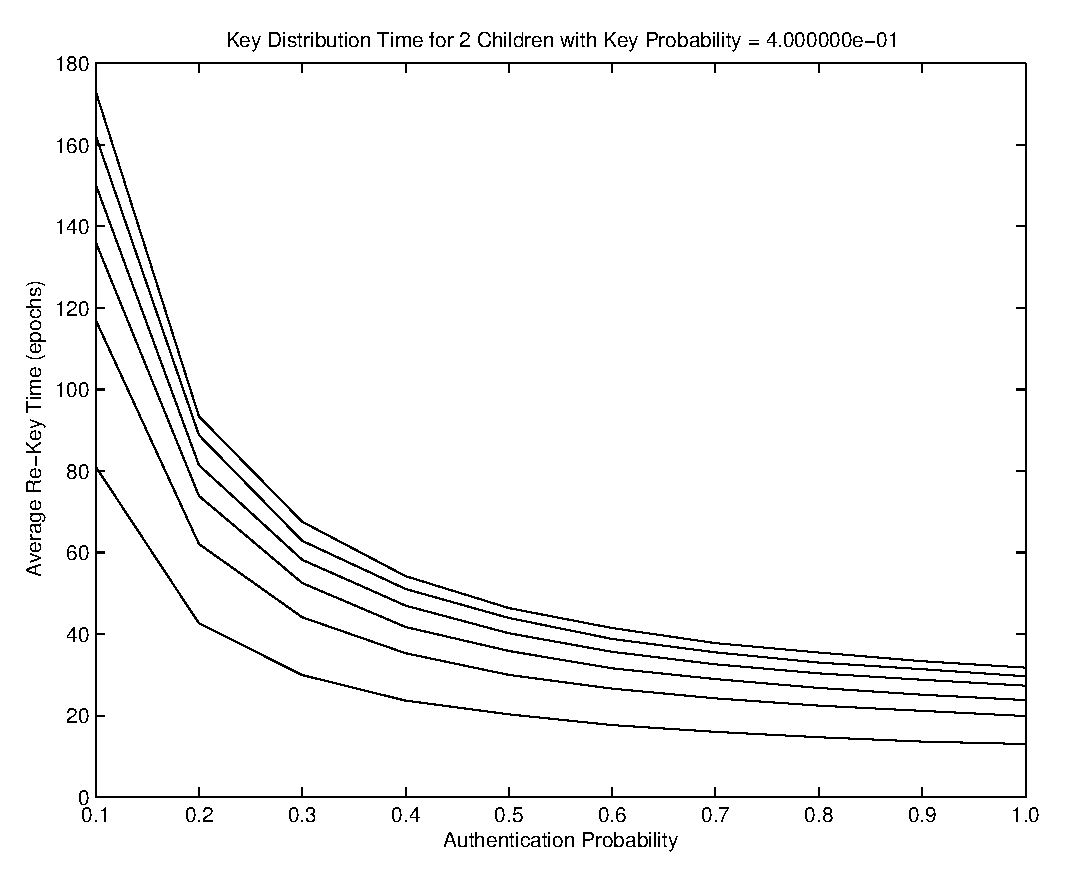
\includegraphics[width=3in]{images_p2/f49.eps} &
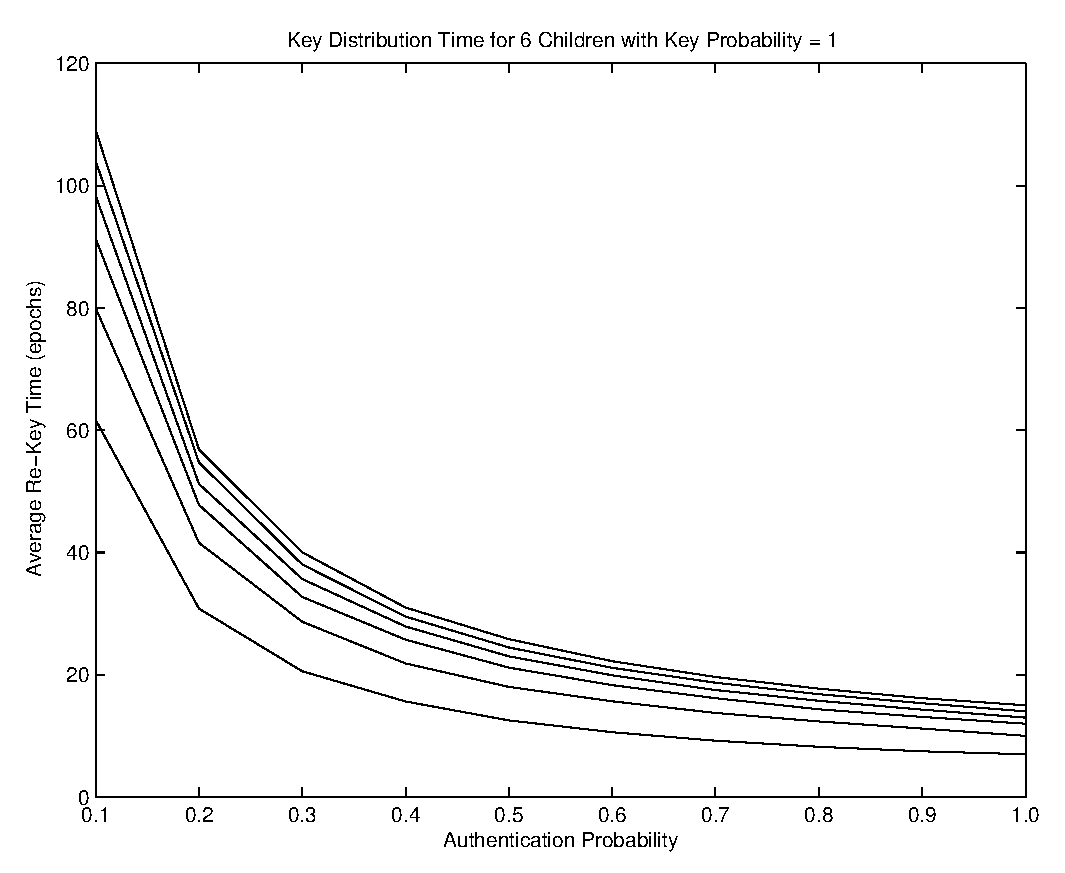
\includegraphics[width=3in]{images_p2/f50.eps}
\end{array}$
\end{center}
\end{figure}
\end{comment}


% That's all folks 
\end{document}
